\documentclass[twoside]{book}

% Packages required by doxygen
\usepackage{calc}
\usepackage{doxygen}
\usepackage{graphicx}
\usepackage[utf8]{inputenc}
\usepackage{makeidx}
\usepackage{multicol}
\usepackage{multirow}
\usepackage{textcomp}
\usepackage[table]{xcolor}

% Font selection
\usepackage[T1]{fontenc}
\usepackage{mathptmx}
\usepackage[scaled=.90]{helvet}
\usepackage{courier}
\usepackage{amssymb}
\usepackage{sectsty}
\renewcommand{\familydefault}{\sfdefault}
\allsectionsfont{%
  \fontseries{bc}\selectfont%
  \color{darkgray}%
}
\renewcommand{\DoxyLabelFont}{%
  \fontseries{bc}\selectfont%
  \color{darkgray}%
}

% Page & text layout
\usepackage{geometry}
\geometry{%
  a4paper,%
  top=2.5cm,%
  bottom=2.5cm,%
  left=2.5cm,%
  right=2.5cm%
}
\tolerance=750
\hfuzz=15pt
\hbadness=750
\setlength{\emergencystretch}{15pt}
\setlength{\parindent}{0cm}
\setlength{\parskip}{0.2cm}
\makeatletter
\renewcommand{\paragraph}{%
  \@startsection{paragraph}{4}{0ex}{-1.0ex}{1.0ex}{%
    \normalfont\normalsize\bfseries\SS@parafont%
  }%
}
\renewcommand{\subparagraph}{%
  \@startsection{subparagraph}{5}{0ex}{-1.0ex}{1.0ex}{%
    \normalfont\normalsize\bfseries\SS@subparafont%
  }%
}
\makeatother

% Headers & footers
\usepackage{fancyhdr}
\pagestyle{fancyplain}
\fancyhead[LE]{\fancyplain{}{\bfseries\thepage}}
\fancyhead[CE]{\fancyplain{}{}}
\fancyhead[RE]{\fancyplain{}{\bfseries\leftmark}}
\fancyhead[LO]{\fancyplain{}{\bfseries\rightmark}}
\fancyhead[CO]{\fancyplain{}{}}
\fancyhead[RO]{\fancyplain{}{\bfseries\thepage}}
\fancyfoot[LE]{\fancyplain{}{}}
\fancyfoot[CE]{\fancyplain{}{}}
\fancyfoot[RE]{\fancyplain{}{\bfseries\scriptsize Generated on Tue Apr 5 2016 20\-:04\-:47 for O\-S\-M area calculation by Doxygen }}
\fancyfoot[LO]{\fancyplain{}{\bfseries\scriptsize Generated on Tue Apr 5 2016 20\-:04\-:47 for O\-S\-M area calculation by Doxygen }}
\fancyfoot[CO]{\fancyplain{}{}}
\fancyfoot[RO]{\fancyplain{}{}}
\renewcommand{\footrulewidth}{0.4pt}
\renewcommand{\chaptermark}[1]{%
  \markboth{#1}{}%
}
\renewcommand{\sectionmark}[1]{%
  \markright{\thesection\ #1}%
}

% Indices & bibliography
\usepackage{natbib}
\usepackage[titles]{tocloft}
\setcounter{tocdepth}{3}
\setcounter{secnumdepth}{5}
\makeindex

% Hyperlinks (required, but should be loaded last)
\usepackage{ifpdf}
\ifpdf
  \usepackage[pdftex,pagebackref=true]{hyperref}
\else
  \usepackage[ps2pdf,pagebackref=true]{hyperref}
\fi
\hypersetup{%
  colorlinks=true,%
  linkcolor=blue,%
  citecolor=blue,%
  unicode%
}

% Custom commands
\newcommand{\clearemptydoublepage}{%
  \newpage{\pagestyle{empty}\cleardoublepage}%
}


%===== C O N T E N T S =====

\begin{document}

% Titlepage & ToC
\hypersetup{pageanchor=false}
\pagenumbering{roman}
\begin{titlepage}
\vspace*{7cm}
\begin{center}%
{\Large O\-S\-M area calculation }\\
\vspace*{1cm}
{\large Generated by Doxygen 1.8.6}\\
\vspace*{0.5cm}
{\small Tue Apr 5 2016 20:04:47}\\
\end{center}
\end{titlepage}
\clearemptydoublepage
\tableofcontents
\clearemptydoublepage
\pagenumbering{arabic}
\hypersetup{pageanchor=true}

%--- Begin generated contents ---
\chapter{Surface-\/sealing}
\label{md_README}
\hypertarget{md_README}{}
\input{md_README}
\chapter{Class Index}
\section{Class List}
Here are the classes, structs, unions and interfaces with brief descriptions\+:\begin{DoxyCompactList}
\item\contentsline{section}{\hyperlink{classNode}{Node} \\*\hyperlink{classNode}{Node} from openstreetmap }{\pageref{classNode}}{}
\end{DoxyCompactList}

\chapter{Class Documentation}
\hypertarget{classNode}{\section{Node Class Reference}
\label{classNode}\index{Node@{Node}}
}


\hyperlink{classNode}{Node} from openstreetmap.  




{\ttfamily \#include $<$Node.\-h$>$}

\subsection*{Public Member Functions}
\begin{DoxyCompactItemize}
\item 
\hyperlink{classNode_aa05b9dee7504eb498c92b42a3b7b4feb}{Node} (unsigned long I\-D, float longitude, float latitude)
\item 
virtual \hyperlink{classNode_aa0840c3cb5c7159be6d992adecd2097c}{$\sim$\-Node} ()
\item 
unsigned long \hyperlink{classNode_a0557c98e510afe0964734b397f2fcd2a}{get\-I\-D} ()
\begin{DoxyCompactList}\small\item\em I\-D-\/getter. \end{DoxyCompactList}\item 
float \hyperlink{classNode_ad6be1e5333414b24f7c3ce59a64b5112}{get\-Longitude} ()
\item 
float \hyperlink{classNode_aa6baaf1097d6196c4cac5f3337adfc7f}{get\-Latitude} ()
\end{DoxyCompactItemize}


\subsection{Detailed Description}
\hyperlink{classNode}{Node} from openstreetmap. 

A class representing a \hyperlink{classNode}{Node} in openstreetmap speaking. It contains the O\-S\-M I\-D of that node, its longitude and its latitude

\begin{DoxyAuthor}{Author}
Stefan 
\end{DoxyAuthor}
\begin{DoxyVersion}{Version}
0.\-1 
\end{DoxyVersion}
\begin{DoxyDate}{Date}
April 02, 2016 
\end{DoxyDate}


\subsection{Constructor \& Destructor Documentation}
\hypertarget{classNode_aa05b9dee7504eb498c92b42a3b7b4feb}{\index{Node@{Node}!Node@{Node}}
\index{Node@{Node}!Node@{Node}}
\subsubsection[{Node}]{\setlength{\rightskip}{0pt plus 5cm}Node\-::\-Node (
\begin{DoxyParamCaption}
\item[{unsigned long}]{I\-D, }
\item[{float}]{longitude, }
\item[{float}]{latitude}
\end{DoxyParamCaption}
)}}\label{classNode_aa05b9dee7504eb498c92b42a3b7b4feb}
Constrtuctor

\begin{DoxyAuthor}{Author}
Stefan 
\end{DoxyAuthor}
\begin{DoxyDate}{Date}
April 2, 2016 
\end{DoxyDate}
\begin{DoxyVersion}{Version}
0.\-1 
\end{DoxyVersion}
\hypertarget{classNode_aa0840c3cb5c7159be6d992adecd2097c}{\index{Node@{Node}!$\sim$\-Node@{$\sim$\-Node}}
\index{$\sim$\-Node@{$\sim$\-Node}!Node@{Node}}
\subsubsection[{$\sim$\-Node}]{\setlength{\rightskip}{0pt plus 5cm}Node\-::$\sim$\-Node (
\begin{DoxyParamCaption}
{}
\end{DoxyParamCaption}
)\hspace{0.3cm}{\ttfamily [virtual]}}}\label{classNode_aa0840c3cb5c7159be6d992adecd2097c}
Destructor

\begin{DoxyAuthor}{Author}
Stefan 
\end{DoxyAuthor}
\begin{DoxyDate}{Date}
April 2, 2016 
\end{DoxyDate}
\begin{DoxyVersion}{Version}
0.\-1 
\end{DoxyVersion}


\subsection{Member Function Documentation}
\hypertarget{classNode_a0557c98e510afe0964734b397f2fcd2a}{\index{Node@{Node}!get\-I\-D@{get\-I\-D}}
\index{get\-I\-D@{get\-I\-D}!Node@{Node}}
\subsubsection[{get\-I\-D}]{\setlength{\rightskip}{0pt plus 5cm}unsigned long Node\-::get\-I\-D (
\begin{DoxyParamCaption}
{}
\end{DoxyParamCaption}
)}}\label{classNode_a0557c98e510afe0964734b397f2fcd2a}


I\-D-\/getter. 

Getter method for the \hyperlink{classNode}{Node}'s I\-D number

\begin{DoxyAuthor}{Author}
Stefan 
\end{DoxyAuthor}
\begin{DoxyDate}{Date}
April 2, 2016 
\end{DoxyDate}
\begin{DoxyVersion}{Version}
0.\-1
\end{DoxyVersion}
\begin{DoxyReturn}{Returns}
I\-D as 64bit integer 
\end{DoxyReturn}
\hypertarget{classNode_aa6baaf1097d6196c4cac5f3337adfc7f}{\index{Node@{Node}!get\-Latitude@{get\-Latitude}}
\index{get\-Latitude@{get\-Latitude}!Node@{Node}}
\subsubsection[{get\-Latitude}]{\setlength{\rightskip}{0pt plus 5cm}float Node\-::get\-Latitude (
\begin{DoxyParamCaption}
{}
\end{DoxyParamCaption}
)}}\label{classNode_aa6baaf1097d6196c4cac5f3337adfc7f}
Getter method for the latitude coordinate. The longitude's format is dd.\-ddddd with sign. North is postive, south is negative.

\begin{DoxyAuthor}{Author}
Stefan 
\end{DoxyAuthor}
\begin{DoxyDate}{Date}
April 2, 2016 
\end{DoxyDate}
\begin{DoxyVersion}{Version}
0.\-1
\end{DoxyVersion}
\begin{DoxyReturn}{Returns}
\hyperlink{classNode}{Node}'s latitude coordinate in dd.\-dddd format as 32bit floating point number 
\end{DoxyReturn}
\hypertarget{classNode_ad6be1e5333414b24f7c3ce59a64b5112}{\index{Node@{Node}!get\-Longitude@{get\-Longitude}}
\index{get\-Longitude@{get\-Longitude}!Node@{Node}}
\subsubsection[{get\-Longitude}]{\setlength{\rightskip}{0pt plus 5cm}float Node\-::get\-Longitude (
\begin{DoxyParamCaption}
{}
\end{DoxyParamCaption}
)}}\label{classNode_ad6be1e5333414b24f7c3ce59a64b5112}
Getter method for the longitude coordinate. The longitude's format is dd.\-ddddd with sign. East is postive, west is negative.

\begin{DoxyAuthor}{Author}
Stefan 
\end{DoxyAuthor}
\begin{DoxyDate}{Date}
April 2, 2016 
\end{DoxyDate}
\begin{DoxyVersion}{Version}
0.\-1
\end{DoxyVersion}
\begin{DoxyReturn}{Returns}
\hyperlink{classNode}{Node}'s longitude coordinate in dd.\-dddd format as 32bit floating point number 
\end{DoxyReturn}


The documentation for this class was generated from the following files\-:\begin{DoxyCompactItemize}
\item 
Node.\-h\item 
Node.\-cpp\end{DoxyCompactItemize}

\hypertarget{structRelatedWay}{\section{Related\-Way Struct Reference}
\label{structRelatedWay}\index{Related\-Way@{Related\-Way}}
}


{\ttfamily \#include $<$Relation.\-h$>$}



Collaboration diagram for Related\-Way\-:
\nopagebreak
\begin{figure}[H]
\begin{center}
\leavevmode
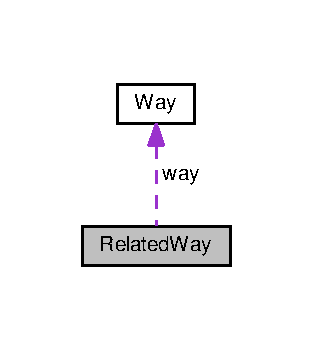
\includegraphics[width=150pt]{structRelatedWay__coll__graph}
\end{center}
\end{figure}
\subsection*{Public Attributes}
\begin{DoxyCompactItemize}
\item 
\hypertarget{structRelatedWay_a5619ada94091c326e4c9440af36a746d}{\hyperlink{classWay}{Way} $\ast$ {\bfseries way}}\label{structRelatedWay_a5619ada94091c326e4c9440af36a746d}

\item 
\hypertarget{structRelatedWay_a92361bcfbff070d7ce5bdcd78193db6e}{char {\bfseries role}}\label{structRelatedWay_a92361bcfbff070d7ce5bdcd78193db6e}

\end{DoxyCompactItemize}


\subsection{Detailed Description}
Struct containing a way and its role as a char to store the content of a \hyperlink{classRelation}{Relation}.

\begin{DoxyAuthor}{Author}
Stefan 
\end{DoxyAuthor}
\begin{DoxyDate}{Date}
April 05,2016 
\end{DoxyDate}
\begin{DoxyVersion}{Version}
0.\-1 
\end{DoxyVersion}


The documentation for this struct was generated from the following file\-:\begin{DoxyCompactItemize}
\item 
Relation.\-h\end{DoxyCompactItemize}

\hypertarget{classRelation}{\section{Relation Class Reference}
\label{classRelation}\index{Relation@{Relation}}
}


O\-S\-M \hyperlink{classRelation}{Relation}.  




{\ttfamily \#include $<$Relation.\-h$>$}

\subsection*{Public Member Functions}
\begin{DoxyCompactItemize}
\item 
\hyperlink{classRelation_a55f2c9d5ae6413cb72c114e583e359ef}{Relation} ()
\begin{DoxyCompactList}\small\item\em Constructor. \end{DoxyCompactList}\item 
virtual \hyperlink{classRelation_ad8bc5c349f9d98b15972fd0b09f341cc}{$\sim$\-Relation} ()
\begin{DoxyCompactList}\small\item\em Destructor. \end{DoxyCompactList}\item 
void \hyperlink{classRelation_ada952e2d9743075b92da916629050733}{add\-Way} (\hyperlink{classWay}{Way} $\ast$way, char role)
\begin{DoxyCompactList}\small\item\em add a way and its role \end{DoxyCompactList}\end{DoxyCompactItemize}


\subsection{Detailed Description}
O\-S\-M \hyperlink{classRelation}{Relation}. 

A class representing a O\-S\-M relation. Relations store several objects, that are related to each other.

\begin{DoxyNote}{Note}
This early version only stores relations between \hyperlink{classWay}{Way} objects
\end{DoxyNote}
\begin{DoxyAuthor}{Author}
Stefan 
\end{DoxyAuthor}
\begin{DoxyDate}{Date}
April 3, 2016 
\end{DoxyDate}
\begin{DoxyVersion}{Version}
0.\-1 
\end{DoxyVersion}


\subsection{Constructor \& Destructor Documentation}
\hypertarget{classRelation_a55f2c9d5ae6413cb72c114e583e359ef}{\index{Relation@{Relation}!Relation@{Relation}}
\index{Relation@{Relation}!Relation@{Relation}}
\subsubsection[{Relation}]{\setlength{\rightskip}{0pt plus 5cm}Relation\-::\-Relation (
\begin{DoxyParamCaption}
{}
\end{DoxyParamCaption}
)}}\label{classRelation_a55f2c9d5ae6413cb72c114e583e359ef}


Constructor. 

Constructor, initializes the object.

\begin{DoxyAuthor}{Author}
Stefan 
\end{DoxyAuthor}
\begin{DoxyDate}{Date}
April 3, 2016 
\end{DoxyDate}
\begin{DoxyVersion}{Version}
0.\-1 
\end{DoxyVersion}
\hypertarget{classRelation_ad8bc5c349f9d98b15972fd0b09f341cc}{\index{Relation@{Relation}!$\sim$\-Relation@{$\sim$\-Relation}}
\index{$\sim$\-Relation@{$\sim$\-Relation}!Relation@{Relation}}
\subsubsection[{$\sim$\-Relation}]{\setlength{\rightskip}{0pt plus 5cm}Relation\-::$\sim$\-Relation (
\begin{DoxyParamCaption}
{}
\end{DoxyParamCaption}
)\hspace{0.3cm}{\ttfamily [virtual]}}}\label{classRelation_ad8bc5c349f9d98b15972fd0b09f341cc}


Destructor. 

Destructor, cleans memory from this object.

\begin{DoxyAuthor}{Author}
Stefan 
\end{DoxyAuthor}
\begin{DoxyDate}{Date}
April 3, 2016 
\end{DoxyDate}
\begin{DoxyVersion}{Version}
0.\-1 
\end{DoxyVersion}


\subsection{Member Function Documentation}
\hypertarget{classRelation_ada952e2d9743075b92da916629050733}{\index{Relation@{Relation}!add\-Way@{add\-Way}}
\index{add\-Way@{add\-Way}!Relation@{Relation}}
\subsubsection[{add\-Way}]{\setlength{\rightskip}{0pt plus 5cm}void Relation\-::add\-Way (
\begin{DoxyParamCaption}
\item[{{\bf Way} $\ast$}]{way, }
\item[{char}]{role}
\end{DoxyParamCaption}
)}}\label{classRelation_ada952e2d9743075b92da916629050733}


add a way and its role 

Adds the I\-D of \hyperlink{classWay}{Way} and maps it to a char, representing the role of the \hyperlink{classWay}{Way}. Adds the \hyperlink{classWay}{Way} to a list of ways in this \hyperlink{classRelation}{Relation}.

\begin{DoxyAuthor}{Author}
Stefan 
\end{DoxyAuthor}
\begin{DoxyDate}{Date}
April 3, 2016 
\end{DoxyDate}
\begin{DoxyVersion}{Version}
0.\-1
\end{DoxyVersion}

\begin{DoxyParams}{Parameters}
{\em way} & The way, that is to be added to the relation \\
\hline
{\em role} & A char representing the role of the \hyperlink{classWay}{Way} way within the relation. The char can be anything, but only 'i' for inner and 'o' for outer will be used. \\
\hline
\end{DoxyParams}


The documentation for this class was generated from the following files\-:\begin{DoxyCompactItemize}
\item 
Relation.\-h\item 
Relation.\-cpp\end{DoxyCompactItemize}

\hypertarget{classWay}{\section{Way Class Reference}
\label{classWay}\index{Way@{Way}}
}


\hyperlink{classWay}{Way} from openstreetmap consisting of connected Nodes.  




{\ttfamily \#include $<$Way.\-h$>$}

\subsection*{Public Member Functions}
\begin{DoxyCompactItemize}
\item 
\hyperlink{classWay_ab4715d81653126b9c799aff81facf800}{Way} (unsigned long I\-D)
\begin{DoxyCompactList}\small\item\em Constructor. \end{DoxyCompactList}\item 
virtual \hyperlink{classWay_aa118212423fa0f1b5c33663e1e0d0b74}{$\sim$\-Way} ()
\begin{DoxyCompactList}\small\item\em Destructor. \end{DoxyCompactList}\item 
unsigned long \hyperlink{classWay_a860214f9a48695b794298c29c829fc40}{get\-I\-D} ()
\begin{DoxyCompactList}\small\item\em I\-D getter. \end{DoxyCompactList}\item 
vector$<$ \hyperlink{classNode}{Node} $\ast$ $>$ $\ast$ \hyperlink{classWay_a690c2eeae8128b5f8d201bba41570d71}{get\-Nodes} ()
\begin{DoxyCompactList}\small\item\em \hyperlink{classNode}{Node} getter. \end{DoxyCompactList}\item 
void \hyperlink{classWay_ada3668577e62311e7c56d2575e5edd00}{add\-Node} (\hyperlink{classNode}{Node} $\ast$node)
\begin{DoxyCompactList}\small\item\em Add a node. \end{DoxyCompactList}\end{DoxyCompactItemize}


\subsection{Detailed Description}
\hyperlink{classWay}{Way} from openstreetmap consisting of connected Nodes. 

A class representing a way of several connected \hyperlink{classNode}{Node} type objects.

\begin{DoxyAuthor}{Author}
Stefan 
\end{DoxyAuthor}
\begin{DoxyDate}{Date}
April 03, 2016 
\end{DoxyDate}
\begin{DoxyVersion}{Version}
0.\-1 
\end{DoxyVersion}


\subsection{Constructor \& Destructor Documentation}
\hypertarget{classWay_ab4715d81653126b9c799aff81facf800}{\index{Way@{Way}!Way@{Way}}
\index{Way@{Way}!Way@{Way}}
\subsubsection[{Way}]{\setlength{\rightskip}{0pt plus 5cm}Way\-::\-Way (
\begin{DoxyParamCaption}
\item[{unsigned long}]{I\-D}
\end{DoxyParamCaption}
)}}\label{classWay_ab4715d81653126b9c799aff81facf800}


Constructor. 

Constructor, initializes the object.

\begin{DoxyAuthor}{Author}
Stefan 
\end{DoxyAuthor}
\begin{DoxyDate}{Date}
April 3, 2016 
\end{DoxyDate}
\begin{DoxyVersion}{Version}
0.\-2 
\end{DoxyVersion}
\hypertarget{classWay_aa118212423fa0f1b5c33663e1e0d0b74}{\index{Way@{Way}!$\sim$\-Way@{$\sim$\-Way}}
\index{$\sim$\-Way@{$\sim$\-Way}!Way@{Way}}
\subsubsection[{$\sim$\-Way}]{\setlength{\rightskip}{0pt plus 5cm}Way\-::$\sim$\-Way (
\begin{DoxyParamCaption}
{}
\end{DoxyParamCaption}
)\hspace{0.3cm}{\ttfamily [virtual]}}}\label{classWay_aa118212423fa0f1b5c33663e1e0d0b74}


Destructor. 

Destructor, cleans up memory.

\begin{DoxyAuthor}{Author}
Stefan 
\end{DoxyAuthor}
\begin{DoxyDate}{Date}
April 3, 2016 
\end{DoxyDate}
\begin{DoxyVersion}{Version}
0.\-1
\end{DoxyVersion}
\begin{DoxyWarning}{Warning}
Deletes the node objects belonging to this way. 
\end{DoxyWarning}


\subsection{Member Function Documentation}
\hypertarget{classWay_ada3668577e62311e7c56d2575e5edd00}{\index{Way@{Way}!add\-Node@{add\-Node}}
\index{add\-Node@{add\-Node}!Way@{Way}}
\subsubsection[{add\-Node}]{\setlength{\rightskip}{0pt plus 5cm}void Way\-::add\-Node (
\begin{DoxyParamCaption}
\item[{{\bf Node} $\ast$}]{node}
\end{DoxyParamCaption}
)}}\label{classWay_ada3668577e62311e7c56d2575e5edd00}


Add a node. 

Add a \hyperlink{classNode}{Node} to the way. The \hyperlink{classNode}{Node} will be contained in the list of nodes for this way after using this operation.

\begin{DoxyAuthor}{Author}
Stefan 
\end{DoxyAuthor}
\begin{DoxyDate}{Date}
April 3, 2016 
\end{DoxyDate}
\begin{DoxyVersion}{Version}
0.\-1
\end{DoxyVersion}

\begin{DoxyParams}{Parameters}
{\em node} & The node to be added \\
\hline
\end{DoxyParams}
\hypertarget{classWay_a860214f9a48695b794298c29c829fc40}{\index{Way@{Way}!get\-I\-D@{get\-I\-D}}
\index{get\-I\-D@{get\-I\-D}!Way@{Way}}
\subsubsection[{get\-I\-D}]{\setlength{\rightskip}{0pt plus 5cm}unsigned long Way\-::get\-I\-D (
\begin{DoxyParamCaption}
{}
\end{DoxyParamCaption}
)}}\label{classWay_a860214f9a48695b794298c29c829fc40}


I\-D getter. 

Getter method for the I\-D number of this \hyperlink{classWay}{Way}.

\begin{DoxyAuthor}{Author}
Stefan 
\end{DoxyAuthor}
\begin{DoxyDate}{Date}
April 3, 2016 
\end{DoxyDate}
\begin{DoxyVersion}{Version}
0.\-1
\end{DoxyVersion}
\begin{DoxyReturn}{Returns}
The I\-D number of that \hyperlink{classWay}{Way} as 64bit integer 
\end{DoxyReturn}
\hypertarget{classWay_a690c2eeae8128b5f8d201bba41570d71}{\index{Way@{Way}!get\-Nodes@{get\-Nodes}}
\index{get\-Nodes@{get\-Nodes}!Way@{Way}}
\subsubsection[{get\-Nodes}]{\setlength{\rightskip}{0pt plus 5cm}vector$<$ {\bf Node} $\ast$ $>$ $\ast$ Way\-::get\-Nodes (
\begin{DoxyParamCaption}
{}
\end{DoxyParamCaption}
)}}\label{classWay_a690c2eeae8128b5f8d201bba41570d71}


\hyperlink{classNode}{Node} getter. 

Getter method for the \hyperlink{classNode}{Node} objects, that belong to this way.

\begin{DoxyAuthor}{Author}
Stefan 
\end{DoxyAuthor}
\begin{DoxyDate}{Date}
April 3, 2016 
\end{DoxyDate}
\begin{DoxyVersion}{Version}
0.\-1
\end{DoxyVersion}
\begin{DoxyReturn}{Returns}
The list of nodes, that belong to this way as std\-::vector$<$\-Node$\ast$$>$
\end{DoxyReturn}
\begin{DoxyWarning}{Warning}
Original list of nodes. 
\end{DoxyWarning}


The documentation for this class was generated from the following files\-:\begin{DoxyCompactItemize}
\item 
Way.\-h\item 
Way.\-cpp\end{DoxyCompactItemize}

%--- End generated contents ---

% Index
\newpage
\phantomsection
\addcontentsline{toc}{chapter}{Index}
\printindex

\end{document}
